\documentclass[]{article}
\usepackage{geometry}
 \geometry{
 a4paper,
 total={170mm,257mm},
 left=20mm,
 top=20mm,
 }
\usepackage{graphicx}
\usepackage{subcaption}

\usepackage[justification=centering]{caption}
\usepackage[hidelinks]{hyperref}
\usepackage{enumitem}
\usepackage[utf8]{inputenc}
\usepackage{float}
\DeclareTextFontCommand{\helvetica}{\fontfamily{phv}\selectfont}
\setlength{\parindent}{4em}
\setlength{\parskip}{1em}
\linespread{1.5}

\usepackage[table]{xcolor}



\title{PAC2  Desenvolupament el treball - Fase 1}
\date{18 de Març 2019}
\author{Vasyl Druchkiv \\ Estudiant de Màster de Bioestadística i Bioinformàtica}
\renewcommand{\contentsname}{Índice}
\usepackage{setspace}

\begin{document}
\maketitle
\makeatletter
\renewcommand{\@seccntformat}[1]{}
\makeatother
\begin{spacing}{0.1}
\tableofcontents
\end{spacing}

L'estructura recomanada per realitzar l'informe de seguiment és la següent:

    \section{Identificació del treball i data de l'informe}

    \section{Descripció de l'avanç del projecte} 

A la data d'avui he desenvolpupat l'aplicació d'anàlisis de les rutes. L'aplicació es completament funcional localment i ofereix l'anàlisi a partir de les bases de dedes GO, KEGG i Reactome. Com estava previst, l'usuari indica l'especie, puja l'arxiu amb els gens i els LogRatios provenents d'estudi de microarrays o NGS. 

L'aplicació està dividira doncs en 4 parts substancials:

\begin{enumerate}
\item Entrada de les dades;
\item Anàlisi GO;
\item Anàlisi KEGG;
\item Anàlisi Reactome.
\end{enumerate}

\begin{figure}[h!]
\caption{Pàgina d'entrada}
\centering
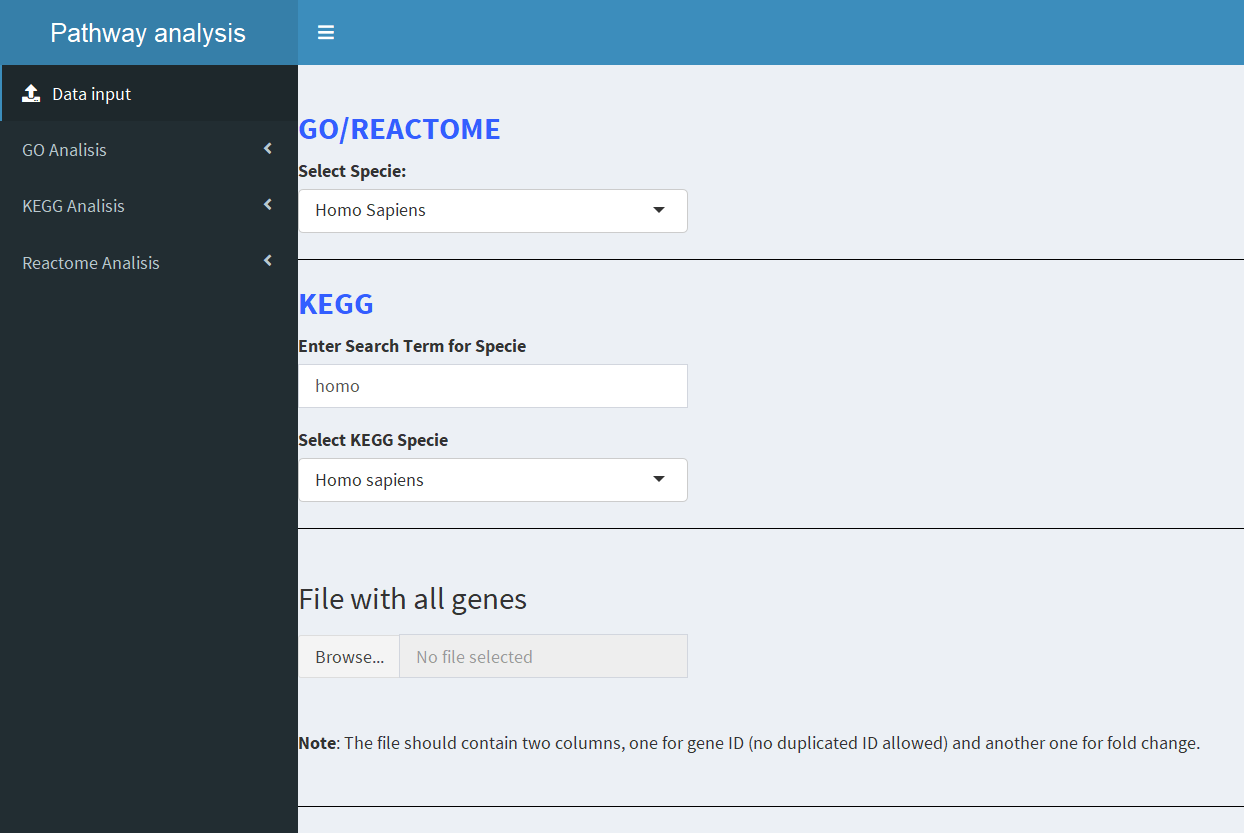
\includegraphics[width=0.9\textwidth]{App_F1}
\end{figure}

L'aplicació ofereix dos mètodes d'anàlisi: d'una banda es pot  fer ORA (Over-Representation Analysis) i d'altra banda l'anàlisi GSEA (Gene Set Enrichment Analisis). Recordem que l'ORA consisteix en selecionar els gens diferencialment expressats i basant-se en GO, KEGG o Reactome comprobar si una de les agrupacións de gens suggerides per aquestes bases de dades està sobre o sotraexpressada en els gens selecionats. Per dur a terme l'ORA l'usuari té opció de definir un \textit{cut-off} de Log-Ratio per formal el conjunt dels gens que s'hi utilitzara (\textit{gene set}). ORA és una bona eina per veure els efectes grans però els effectes petits li escapen.  Els efectes petits derivats dels gens individuals poden acommular-se en un efect conjunt substancial el qual ORA no serà capaç de detectar. És aquí on GSEA mostra la seva utilitat. 

     \subsection{Grau de compliment dels objectius i resultats previstos en el pla de treball.}

Primer recordem les tasques proposats a la PAC1:

\begin{figure}[h!]
\caption{Calendàri}
\centering
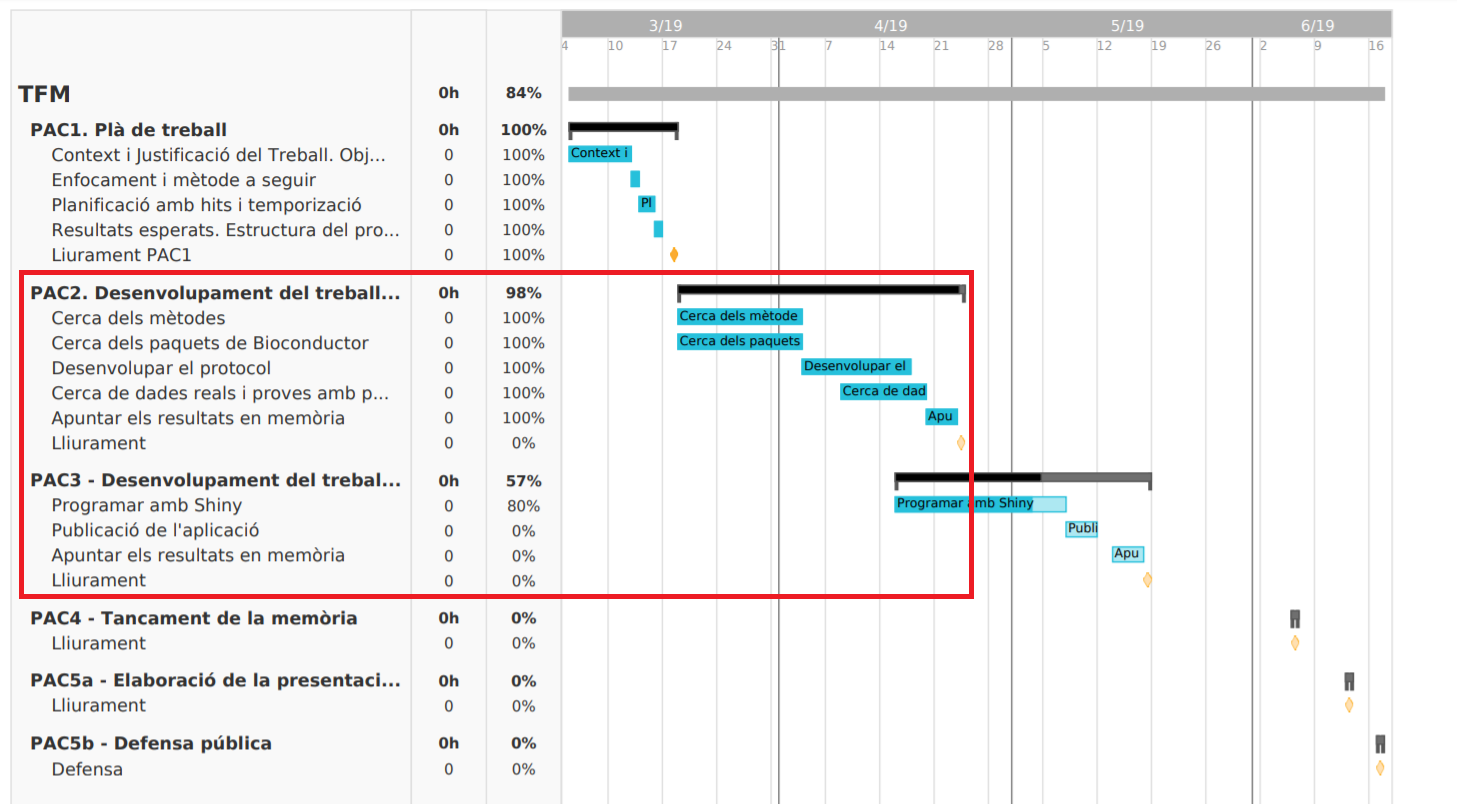
\includegraphics[width=0.9\textwidth]{Calender}
\end{figure}

     \subsection{Justificació dels canvis en cas necessari}

   \section{Relació de les activitats realitzades}

         \subsection{Activitats previstes en el pla de treball}

         \subsection{Activitats no previstes i realitzades o programes}

   \section{Relació de les desviacions en la temporització i accions de mitigació si escau i actualització del cronograma si escau}

   \section{Llistat dels resultats parcials obtinguts fins al moment (lliurables que s'adjunten)}

   \section{Comentaris del vostre director particular si ho considereu necessari.}

\end{document}





































